\documentclass{beamer}

%-----------------------
%% This template is based on a template developed by the SMCS
%% (Statistical Methodology and Computing Service) at UCLouvain

%-----------------------
% pour faire les slides papiers :
% \documentclass[handout, compress]{beamer}
% \usepackage{pgfpages}
% % 4 par page
% \pgfpagesuselayout{4 on 1}[a4paper,border shrink=5mm, landscape]
% % 2 par page
% \pgfpagesuselayout{2 on 1}[a4paper,border shrink=5mm]

\usetheme{UCL2018}

\usepackage[utf8]{inputenc}
\usepackage[T1]{fontenc}
\usepackage{lmodern}
\usepackage{xspace}
\usepackage{float}
\usepackage{graphicx}
\usepackage{amssymb}
\usepackage{hyperref}
\usepackage{ragged2e}
\usepackage[authoryear, round]{natbib}

%% For slides in French
%% \usepackage[french]{babel}
%% \usepackage[cyr]{aeguill}

\usepackage{lipsum}

\theoremstyle{example}
\newtheorem{examplef}{Example}
\newtheorem{examplesf}{Examples}
\newcommand{\ei}{\end{itemize}}

\usepackage{xmpincl}

\newcommand{\sidebysidecaption}[4]{%
\RaggedRight%
  \begin{minipage}[t]{#1}
    \vspace*{0pt}
    #3
  \end{minipage}
  \hfill%
  \begin{minipage}[t]{#2}
    \vspace*{0pt}
    #4
\end{minipage}%
}


\title{Probabilistic mapping  of the sub-cellular proteome}
\author[]{Laurent Gatto}
\date{13 February 2020}
\institute[]{CBIO, de Duve Institute, UCLouvain}
\subtitle{Slides available at: \url{http://bit.ly/ABLS2020}}


\begin{document}

\pdfinfo {/Author(Laurent Gatto - UCLouvain)}

%-----------------------------------------------
% Abstract
%-----------------------------------------------

%% Abstract: In biology, localisation is function - understanding the
%% sub-cellular localisation of proteins is paramount to comprehend
%% the context and full extend of their functions. Shotgun mass
%% spectrometry-based spatial proteomics method are orthogonal to
%% widely used targeted microscopy-based assay. In conjunction with
%% contemporary machine learning, the former enable to build
%% proteome-wide protein localisation maps, informing us on the
%% location of thousands of proteins. When studying these
%% proteome-wide spatial maps, one can learn that while some proteins
%% can be found in a single location within a cell, up to half of the
%% proteins may reside in multiple locations, can dynamically
%% re-localise, or reside within an unknown functional compartment,
%% leading to considerable uncertainty in associating proteins to
%% their sub-cellular location. Recent Bayesian modelling approaches
%% enable us to mine these data, and in particular the dynamic
%% fraction of the spatial proteome, in much greater depth. We are now
%% in a position to (1) probabilistically model protein localisation
%% as well as quantify the uncertainty in the location assignments,
%% and (2) compute a probability for, and quantify uncertainty in,
%% whether a protein is differentially localised upon cellular
%% perturbation. These computational approaches lead to better and
%% more trustworthy biological interpretation of these rich spatial
%% proteomics data.

%-----------------------------------------------
% Title page
%-----------------------------------------------


\begin{frame}[plain]
\titlepage
\end{frame}


\begin{frame}{Acknowledgements}


\textcolor{Blue}{Dr Lisa Breckels}, Cambridge: novelty detection,
transfer learning, \texttt{pRoloc} and \texttt{pRolocdata}.

\bigskip

\textcolor{Blue}{Mr Oliver Crook}, Cambridge: Bayesian spatial
proteomics, \texttt{pRoloc} and \texttt{pRolocdata}.

\bigskip

Funding: BBSRC, Wellcome Trust

\end{frame}


%-----------------------------------------------
% Table of content
%-----------------------------------------------

\AtBeginSection[]{
  \setbeamercolor{background canvas}{bg=UCLblue2}
  \setbeamercolor{section in toc}{fg=UCLblue}
  \setbeamercolor{subsection in toc}{fg=UCLblue}
  \setbeamerfont{section in toc}{size=\large}

  \mode<handout>{
    \setbeamercolor{background canvas}{bg=white}
    \setbeamercolor{section in toc}{fg=UCLblue}
    \setbeamercolor{subsection in toc}{fg=UCLblue}
  }

  \begin{frame}[plain]
    \frametitle{Outline}
    \tableofcontents[currentsection,hideothersubsections]
  \end{frame}

  \setbeamercolor{background canvas}{bg=white}
}


%-----------------------------------------------
% Content
%-----------------------------------------------

\section{Spatial proteomics}


\begin{frame}{Cell organisation - \textbf{localisation is function}}
  \begin{center}
    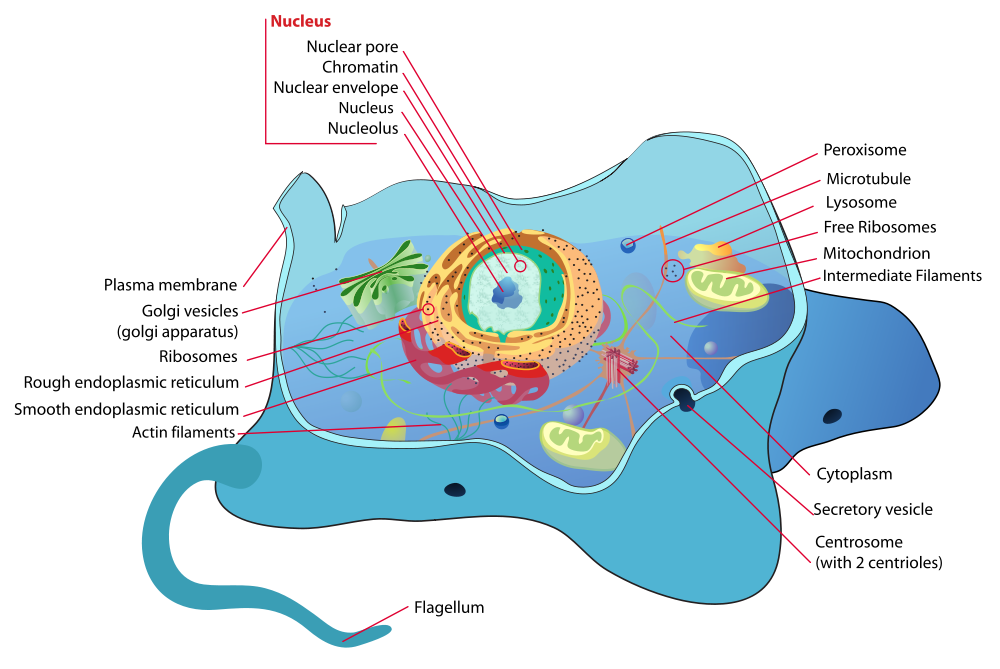
\includegraphics[width=.8\linewidth]{figs/Animal_cell_structure.png} \\
    \textbf{\textcolor{Blue}{Spatial proteomics}} is the systematic
    study of protein localisations.
  \end{center}

  \begin{center}
    \textbf{Localisation -- re-localisation -- mis-localisation}
  \end{center}

  \tiny Image from Wikipedia
  \url{http://en.wikipedia.org/wiki/Cell_(biology)}.
\end{frame}


%% \begin{frame}{Spatial proteomics - Why?}

%%   \begin{itemize}

%%   \item \textbf{Localisation is function}: Localisation and
%%     sequestration of proteins within sub-cellular niches is a
%%     fundamental mechanism for the post-translational regulation of
%%     protein function.

%%     \bigskip

%%   \item \textbf{Re-localisation}: \textcolor{Blue}{differentiation}
%%     stem cells, \textcolor{Blue}{activation} of biological processes.

%%     \bigskip

%%   \item \textbf{Mis-localisation}: Disruption of the
%%     targeting/trafficking process alters proper sub-cellular
%%     localisation, which in turn perturb the cellular functions of the
%%     proteins.

%%   \end{itemize}

%% \end{frame}


\begin{frame}{}

  \begin{columns}
    \begin{column}{0.5\textwidth}

      \textbf{Explorative/discovery approaches},
      \textcolor{Blue}{steady-state \textbf{global localisation maps}}
      (as opposed to microscopy-based targeted approaches).

      \bigskip

      \small{

        \textbf{Density gradient}: PCP \citep{Dunkley:2006}, LOPIT
        \citep{Foster2006}, hyperLOPIT
        \citep{Christoforou:2016,Mulvey:2017} and \\

        \textbf{Differential centrifugation} \cite{Itzhak:2016},
        LOPIT-DC \citep{Geladaki:2019}.

      }

      \bigskip


    \end{column}
    \begin{column}{0.5\textwidth}
      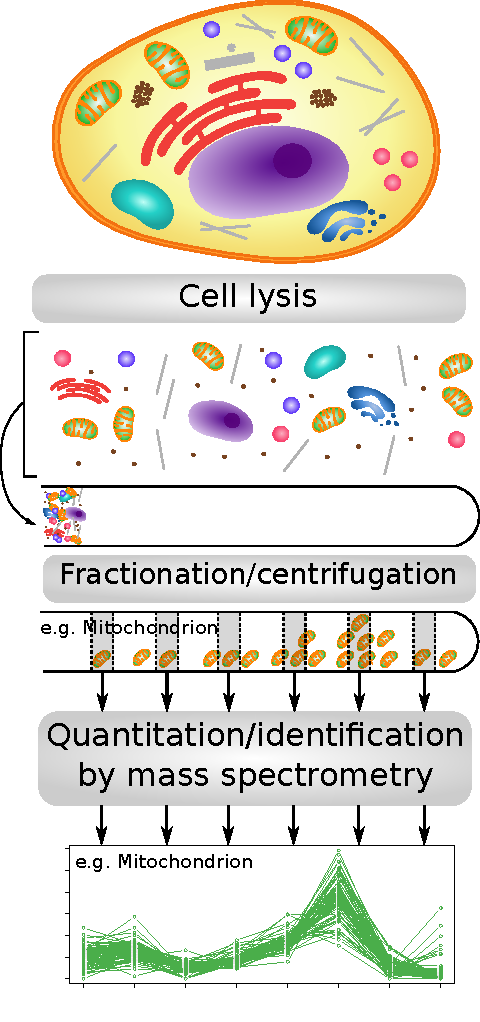
\includegraphics[width=.78\linewidth]{figs/workflow_primary.pdf}
    \end{column}
  \end{columns}

\end{frame}

\subsubsection*{The data}
\label{sec:data}

\begin{frame}{Quantitation data}
  \begin{center}
    \begin{tabular}{|l|llll|}
      \hline
      & Fraction$_{\text{1}}$ & Fraction$_{\text{2}}$ & \ldots{} & Fraction$_{\text{L}}$ \\
      \hline
      {\bf x}$_{\text{1}}$ & $x_{\text{1,1}}$ & $x_{\text{1,2}}$ & \ldots{} & $x_{\text{1,L}}$ \\
      {\bf x}$_{\text{2}}$ & $x_{\text{2,1}}$ & $x_{\text{2,2}}$ & \ldots{} & $x_{\text{2,L}}$ \\
      {\bf x}$_{\text{3}}$ & $x_{\text{3,1}}$ & $x_{\text{3,2}}$ & \ldots{} & $x_{\text{3,L}}$ \\
      \vdots & \vdots & \vdots & \vdots & \vdots \\
      {\bf x}$_{\text{i}}$ & $x_{\text{i,1}}$ & $x_{\text{i,2}}$ & \ldots{} & $x_{\text{i,L}}$ \\
      \vdots & \vdots & \vdots & \vdots & \vdots \\
      {\bf x}$_{\text{N}}$ & $x_{\text{N,1}}$ & $x_{\text{N,2}}$ & \ldots{} & $x_{\text{N, L}}$ \\
      \hline
    \end{tabular}
  \end{center}
\end{frame}

\begin{frame}{Quantitation data and organelle markers}
  \begin{center}
    \begin{tabular}{|l|llll||l|}
      \hline
      & Fraction$_{\text{1}}$ & Fraction$_{\text{2}}$ & \ldots{} & Fraction$_{\text{L}}$ & markers\\
      \hline
      {\bf x}$_{\text{1}}$ & $x_{\text{1,1}}$ & $x_{\text{1,2}}$ & \ldots{} & $x_{\text{1,L}}$ & unknown \\
      {\bf x}$_{\text{2}}$ & $x_{\text{2,1}}$ & $x_{\text{2,2}}$ & \ldots{} & $x_{\text{2,L}}$ & \textcolor{Red}{$loc_{1}$}\\
      {\bf x}$_{\text{3}}$ & $x_{\text{3,1}}$ & $x_{\text{3,2}}$ & \ldots{} & $x_{\text{3,L}}$ & unknown \\
      \vdots & \vdots & \vdots & \vdots & \vdots & \vdots \\
      {\bf x}$_{\text{i}}$ & $x_{\text{i,1}}$ & $x_{\text{i,2}}$ & \ldots{} & $x_{\text{i,L}}$ & \textcolor{Blue}{$loc_{k}$}\\
      \vdots & \vdots & \vdots & \vdots & \vdots & \vdots\\
      {\bf x}$_{\text{N}}$ & $x_{\text{N,1}}$ & $x_{\text{N,2}}$ & \ldots{} & $x_{\text{N, K}}$ & unknown \\
      \hline
    \end{tabular}
  \end{center}
\end{frame}


%-----------------------------------------------
% New section
%-----------------------------------------------

\section{Data analysis (1)}


\begin{frame}{Visualisation}
  \begin{figure}
    \centering
    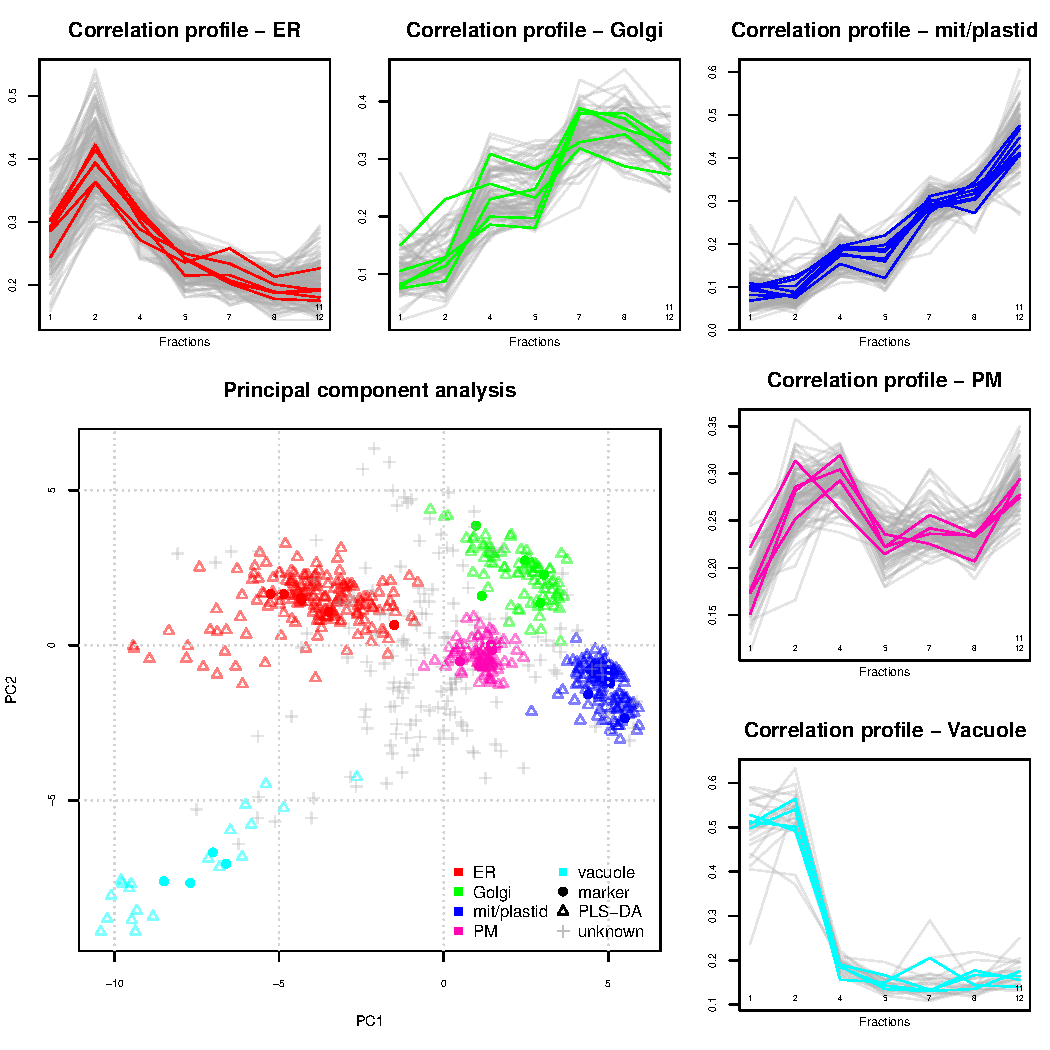
\includegraphics[width=.6\linewidth]{figs/F04-analyses.pdf}
    \caption{From \cite{Gatto:2010}, \textit{Arabidopsis thaliana} data
      from \cite{Dunkley:2006}}
  \end{figure}
\end{frame}

\begin{frame}{Quality control}
  \begin{figure}
    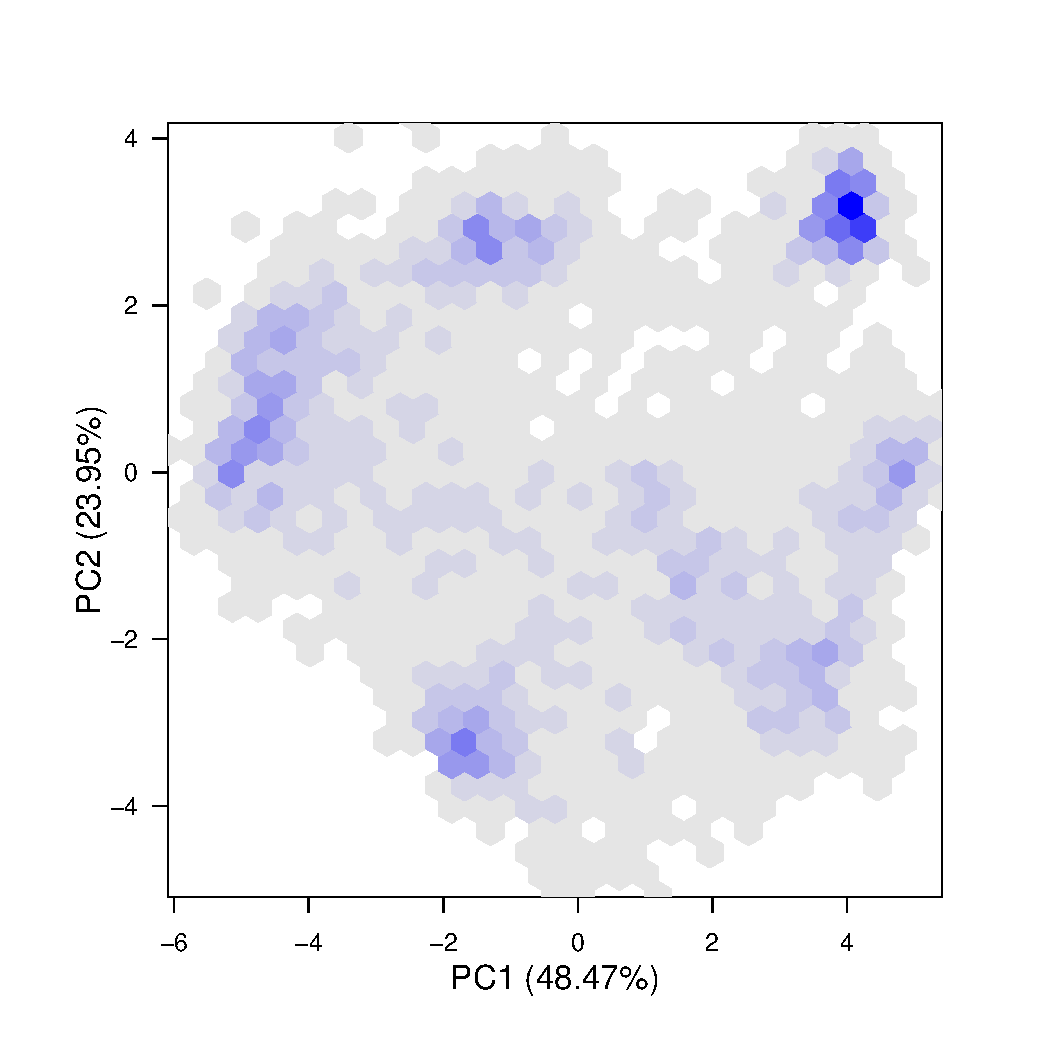
\includegraphics[width=.32\linewidth]{figs/hex1.pdf}
    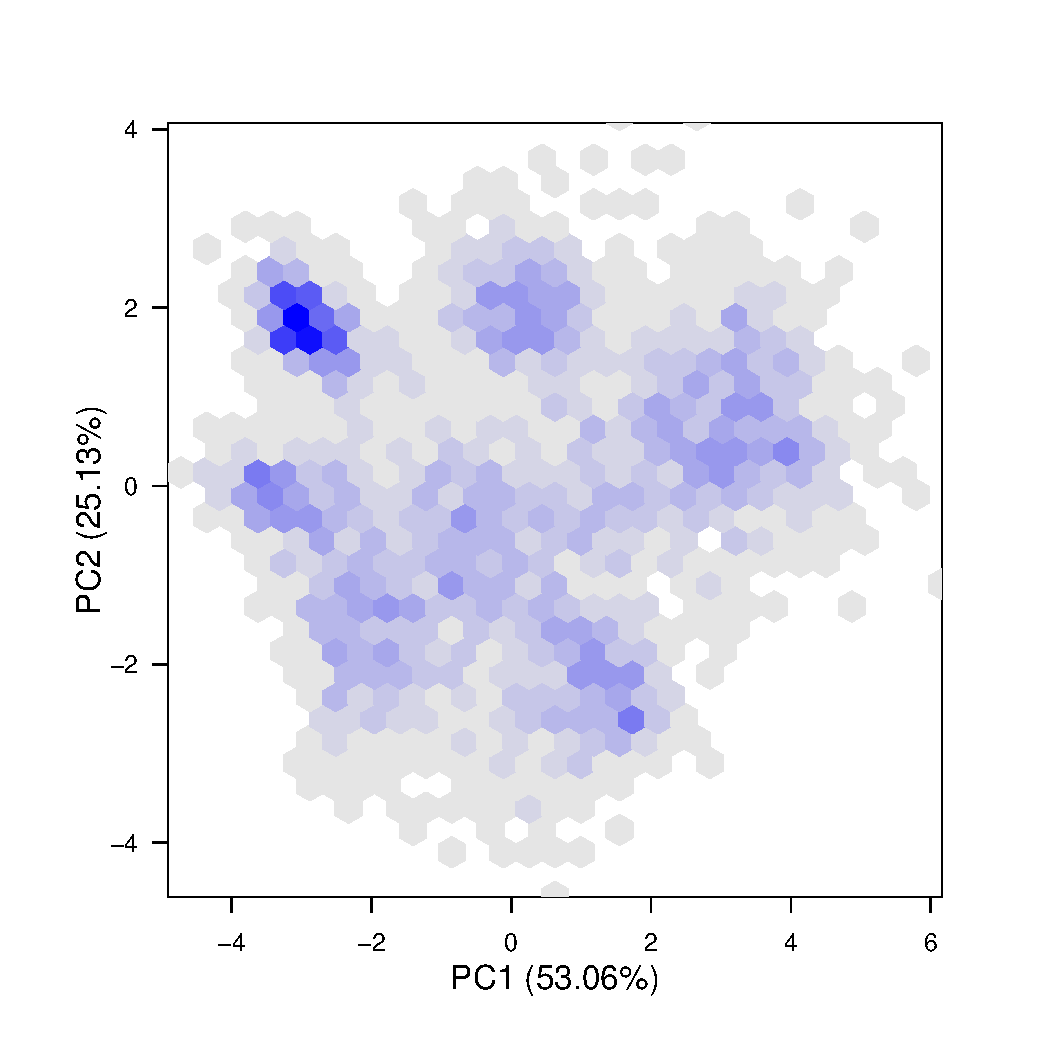
\includegraphics[width=.32\linewidth]{figs/hex2.pdf}
    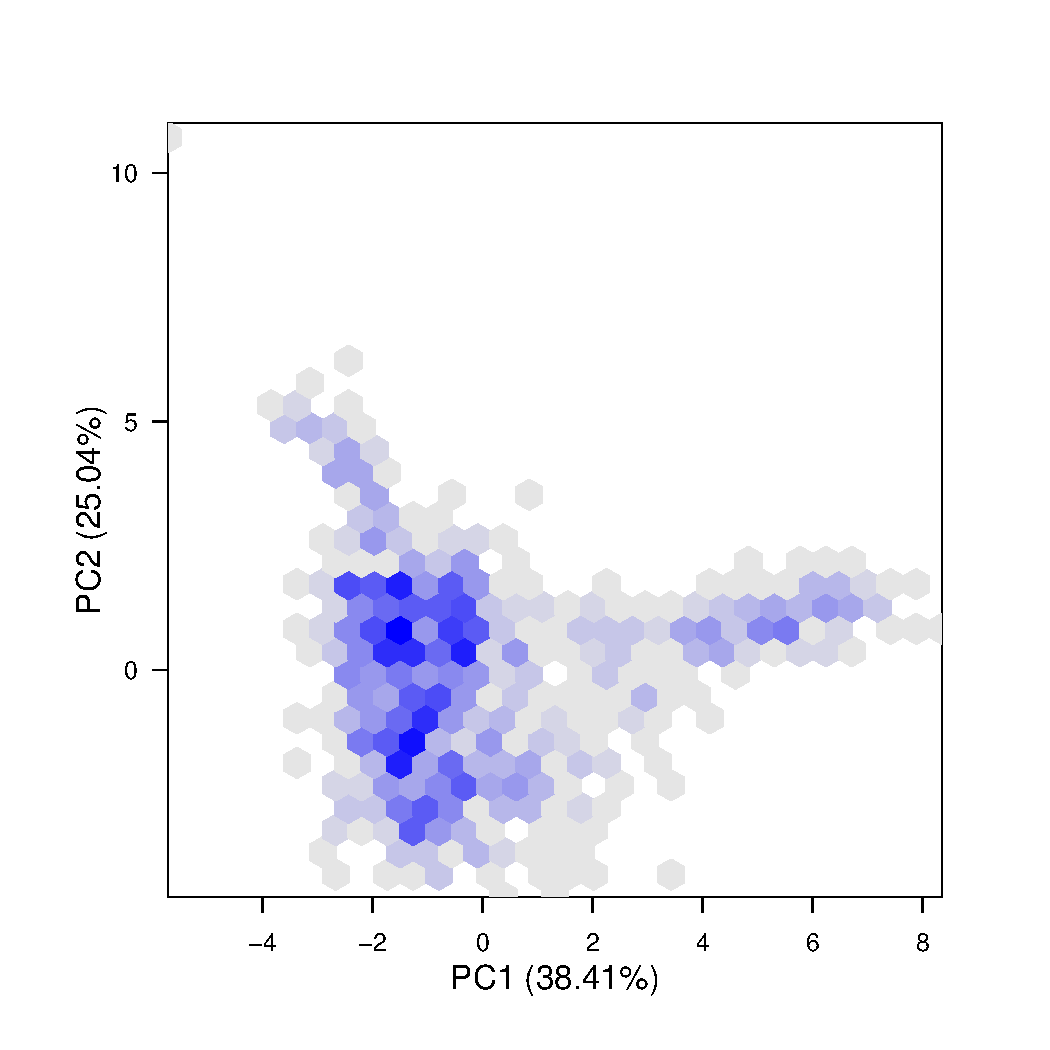
\includegraphics[width=.32\linewidth]{figs/hex3.pdf}
    \caption{Assessing sub-cellular resolution in spatial proteomics
      experiments \citep{Gatto:2018}}
  \end{figure}
\end{frame}


\begin{frame}{Problem statement: classification}
  \begin{figure}[h]
    \centering
    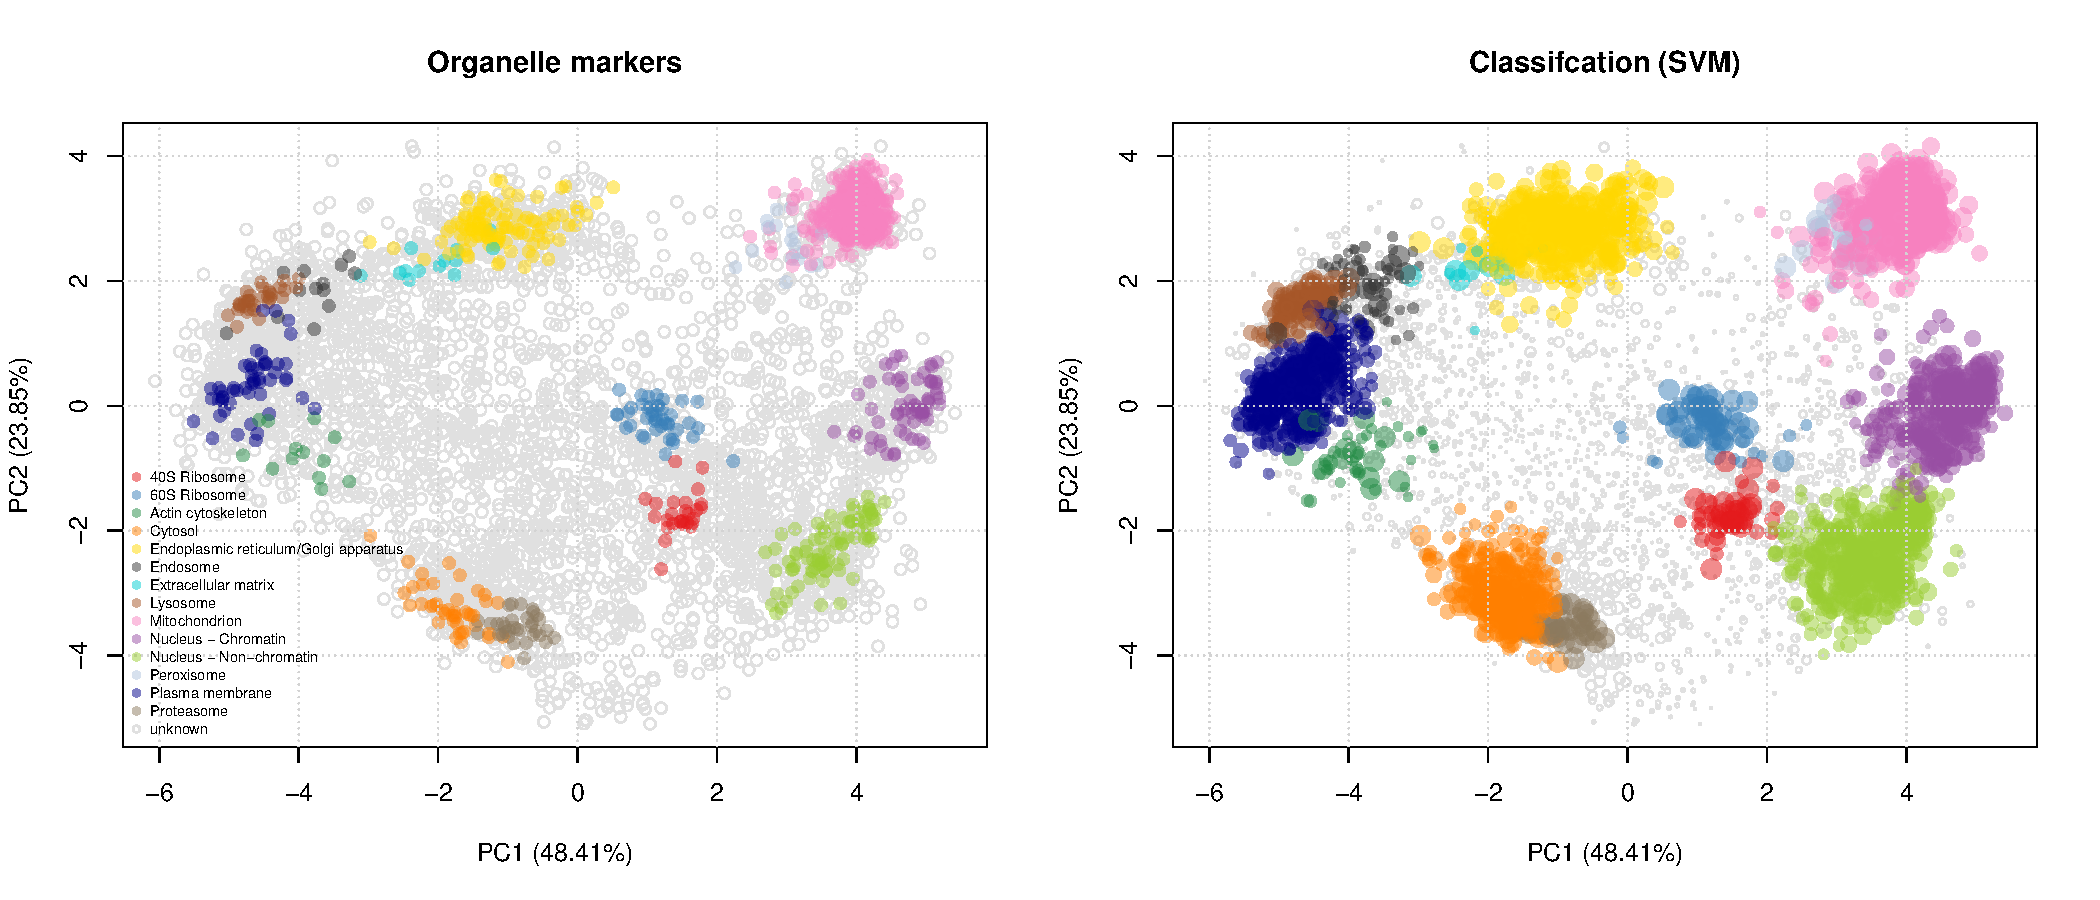
\includegraphics[width=\linewidth]{figs/hyperlopit-class.pdf}
    \caption{Support vector machines classifier (after 5\% FDR
      classification cutoff) on the embryonic stem cell data from
      \cite{Christoforou:2016}.}
  \end{figure}
\end{frame}


\begin{frame}{Computational challenges}

  \begin{itemize}
  \item Visualisation (cluster, unsupervised learning)
  \item Classification (supervised learning)
  \item \textbf{Novelty detection} (semi-supervised learning)
  \item Data integration (transfer learning)
  \item \textbf{Unvertainty quantification}
  \item \textbf{Multi-localisation}
  \item \textbf{Spatial dynamics}
  \end{itemize}
  \centering

  \bigskip

  {\Large To uncover and understand biology}
\end{frame}


%-----------------------------------------------
% New section
%-----------------------------------------------

\section{Computational spatial proteomics (2)}

\subsection{Novelty detection}


\begin{frame}{Importance of annotation}

  \begin{columns}[t]
    \begin{column}[T]{0.43\textwidth}
      \begin{centering}
        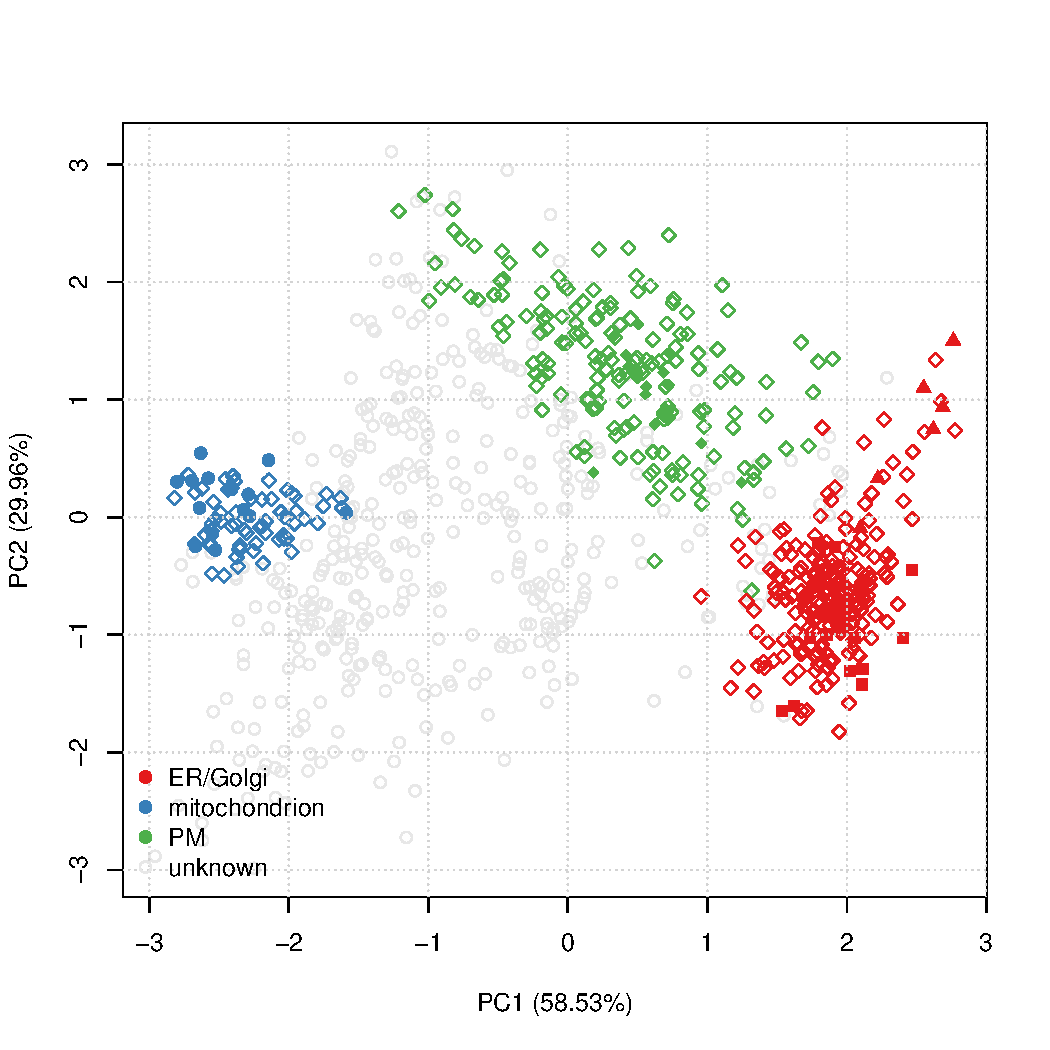
\includegraphics[width=1\linewidth]{figs/tan2009r1org.pdf}
      \end{centering}
    \end{column}
    \begin{column}[T]{0.56\textwidth}
      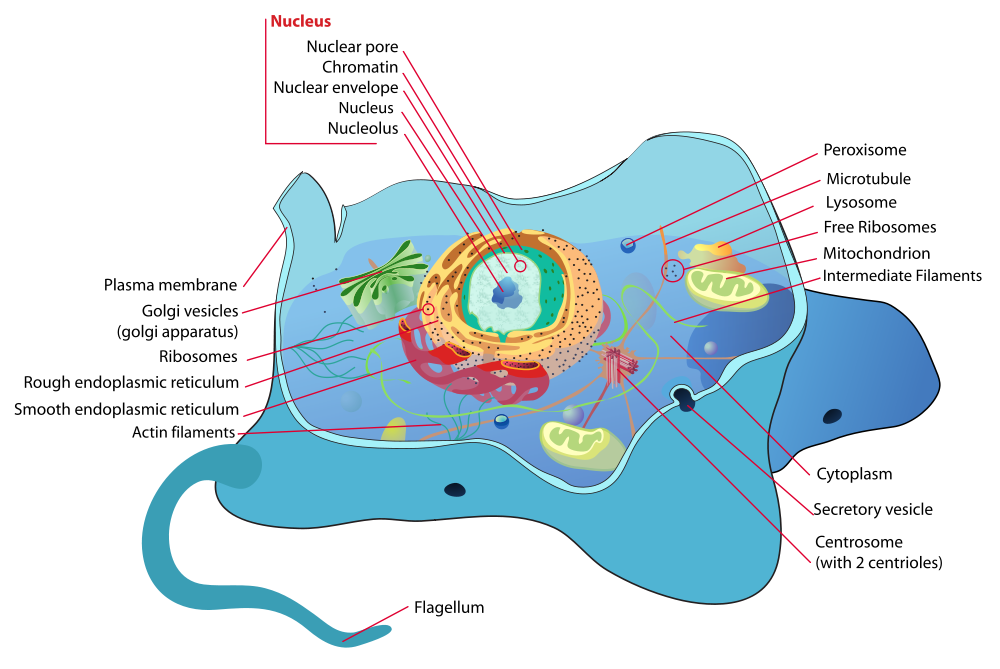
\includegraphics[width=1\linewidth]{figs/Animal_cell_structure.png}
    \end{column}
  \end{columns}
  Incomplete annotation, and therefore lack of training data, for
  many/most organelles. \textit{Drosophila} data from \cite{Tan2009}.
\end{frame}

\begin{frame}{Semi-supervised learning: novelty detection}
  \begin{figure}
    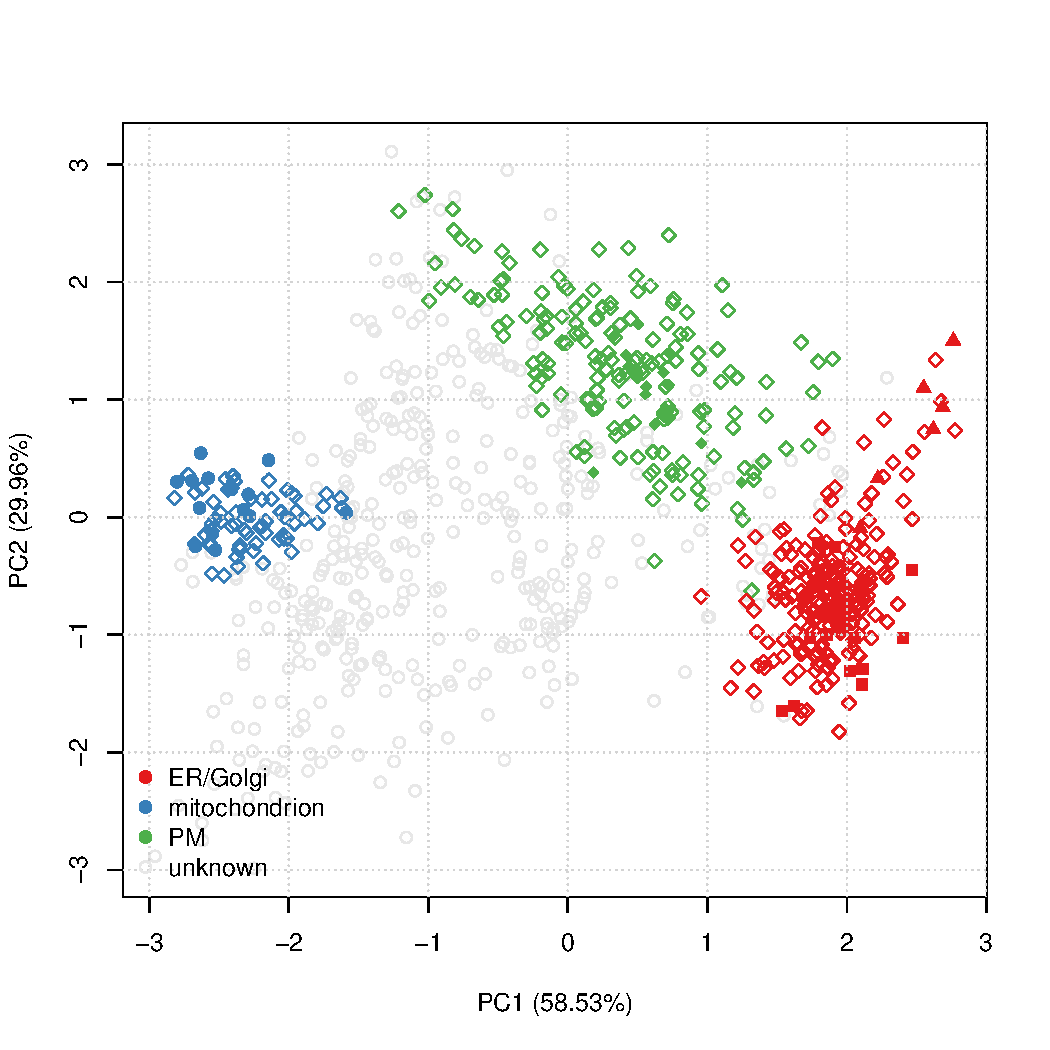
\includegraphics[width=.48\linewidth]{figs/tan2009r1org.pdf}
    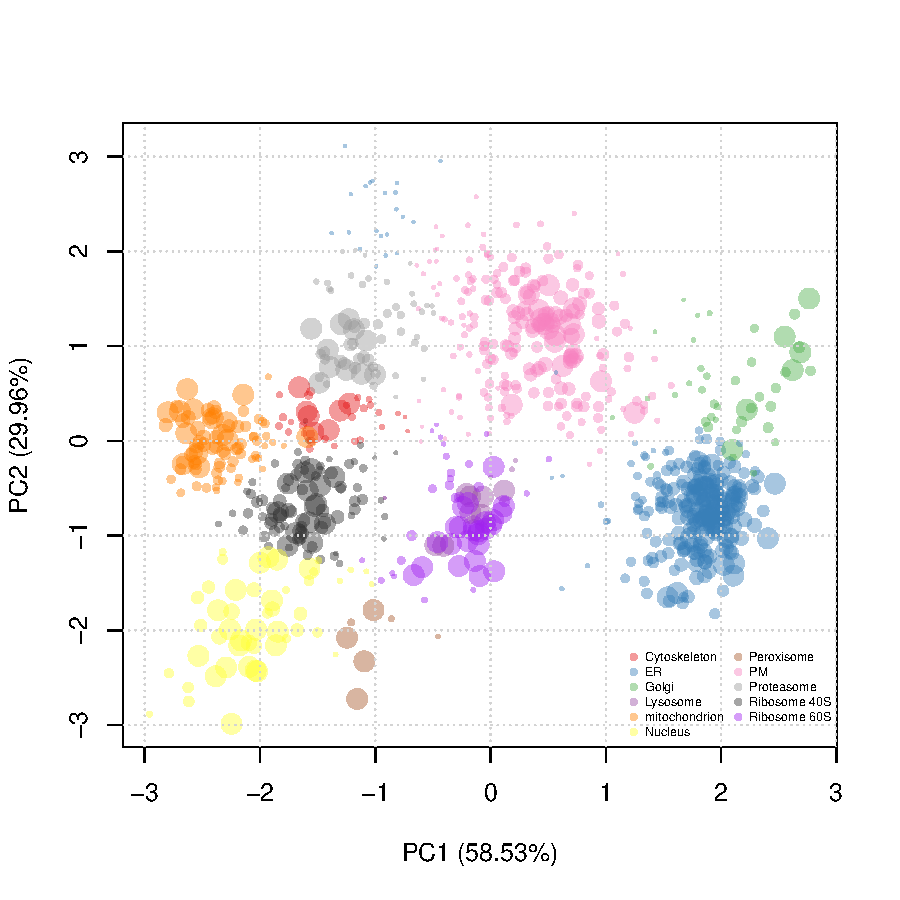
\includegraphics[width=.5\linewidth]{figs/pdres2fig.pdf}
    \caption{Left: Original \textit{Drosophila} data from
      \cite{Tan2009}. Right: After semi-supervised learning and
      classification, \cite{Breckels:2013}. Under development:
      Bayesian novelty detection (Novelty-TAGM, see below).}
  \end{figure}
\end{frame}


%-----------------------------------------------
% New section
%-----------------------------------------------

\subsection{Multi-localisation and uncertainly quantification}

\begin{frame}{How much do we learn? How much do we miss?}
  \begin{figure}
    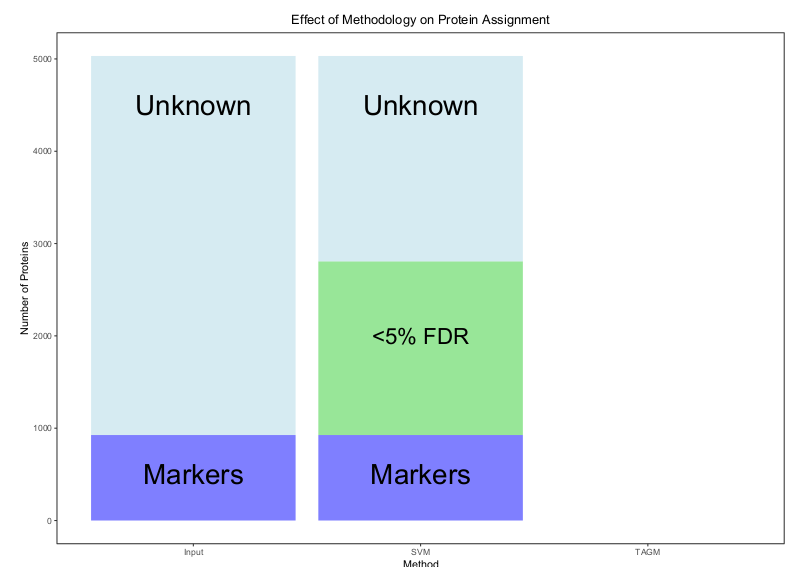
\includegraphics[width=.8\linewidth]{./figs/preConcludePlot.png}
  \end{figure}
\end{frame}


\begin{frame}{Bayesian Mixture Modelling For Spatial Proteomics}

  \begin{itemize}

    \item<+-> \textit{T Augmented Gaussian Mixture model (TAGM)} is a
      \textbf{multivariate Gaussian generative model} for MS-based
      spatial proteomics data. It posits that each annotated
      sub-cellular niche can be modelled by a multivariate Gaussian
      distribution.

    \item<+-> With the prior knowledge that many proteins are not
      captured by known sub-cellular niches, we augment our model with
      an \textbf{outlier component}. Outliers are often dispersed and
      thus this additional component is described by a heavy-tailed
      distribution: the multivariate Student's t-distribution, leading
      us to a \textit{T Augmented Gaussian Mixture model}
      \citep{Crook:2018,Crook:2019}.

    \item<+-> This methodology allows proteome-wide
      \textbf{uncertainty quantification}, thus adding a further layer
      to the analysis of spatial proteomics.

  \end{itemize}
\end{frame}


\begin{frame}{}

    We initially model the distribution of profiles associated with
    proteins that localise to the $k$-th component as multivariate
    normal with mean vector $\boldsymbol{\mu}_k$ and covariance matrix
    $\Sigma_k$, so that:

    \begin{align}
      {\bf x}_i | z_i = k \quad \sim \mathcal{N}(\boldsymbol{\mu}_k, \Sigma_k) \label{equation::preq}
    \end{align}

    \pause

    We extend it by introducing an additional \textit{outlier
      component}. To do this, we augment our model by introducing a
    further indicator latent variable $\phi$. Each protein ${\bf x}_i$
    is now described by an additional variable $\phi_i$, with $\phi_i
    = 1$ indicating that protein ${\bf x}_i$ belongs to a organelle
    derived component and $\phi_i = 0$ indicating that protein ${\bf
      x}_i$ is not well described by these known components. This
    outlier component is modelled as a multivariate T distribution
    with degrees of freedom $\kappa$, mean vector $\bf{M}$, and scale
    matrix $V$.

    \begin{align}
      {\bf x}_i | z_i = k, \phi_i \quad \sim \mathcal{N}(\boldsymbol{\mu}_k, \Sigma_k)^{\phi_i}\mathcal{T}(\kappa, \boldsymbol{M}, V)^{1 - \phi_i }
    \end{align}


\end{frame}


\begin{frame}{}
      \begin{figure}
        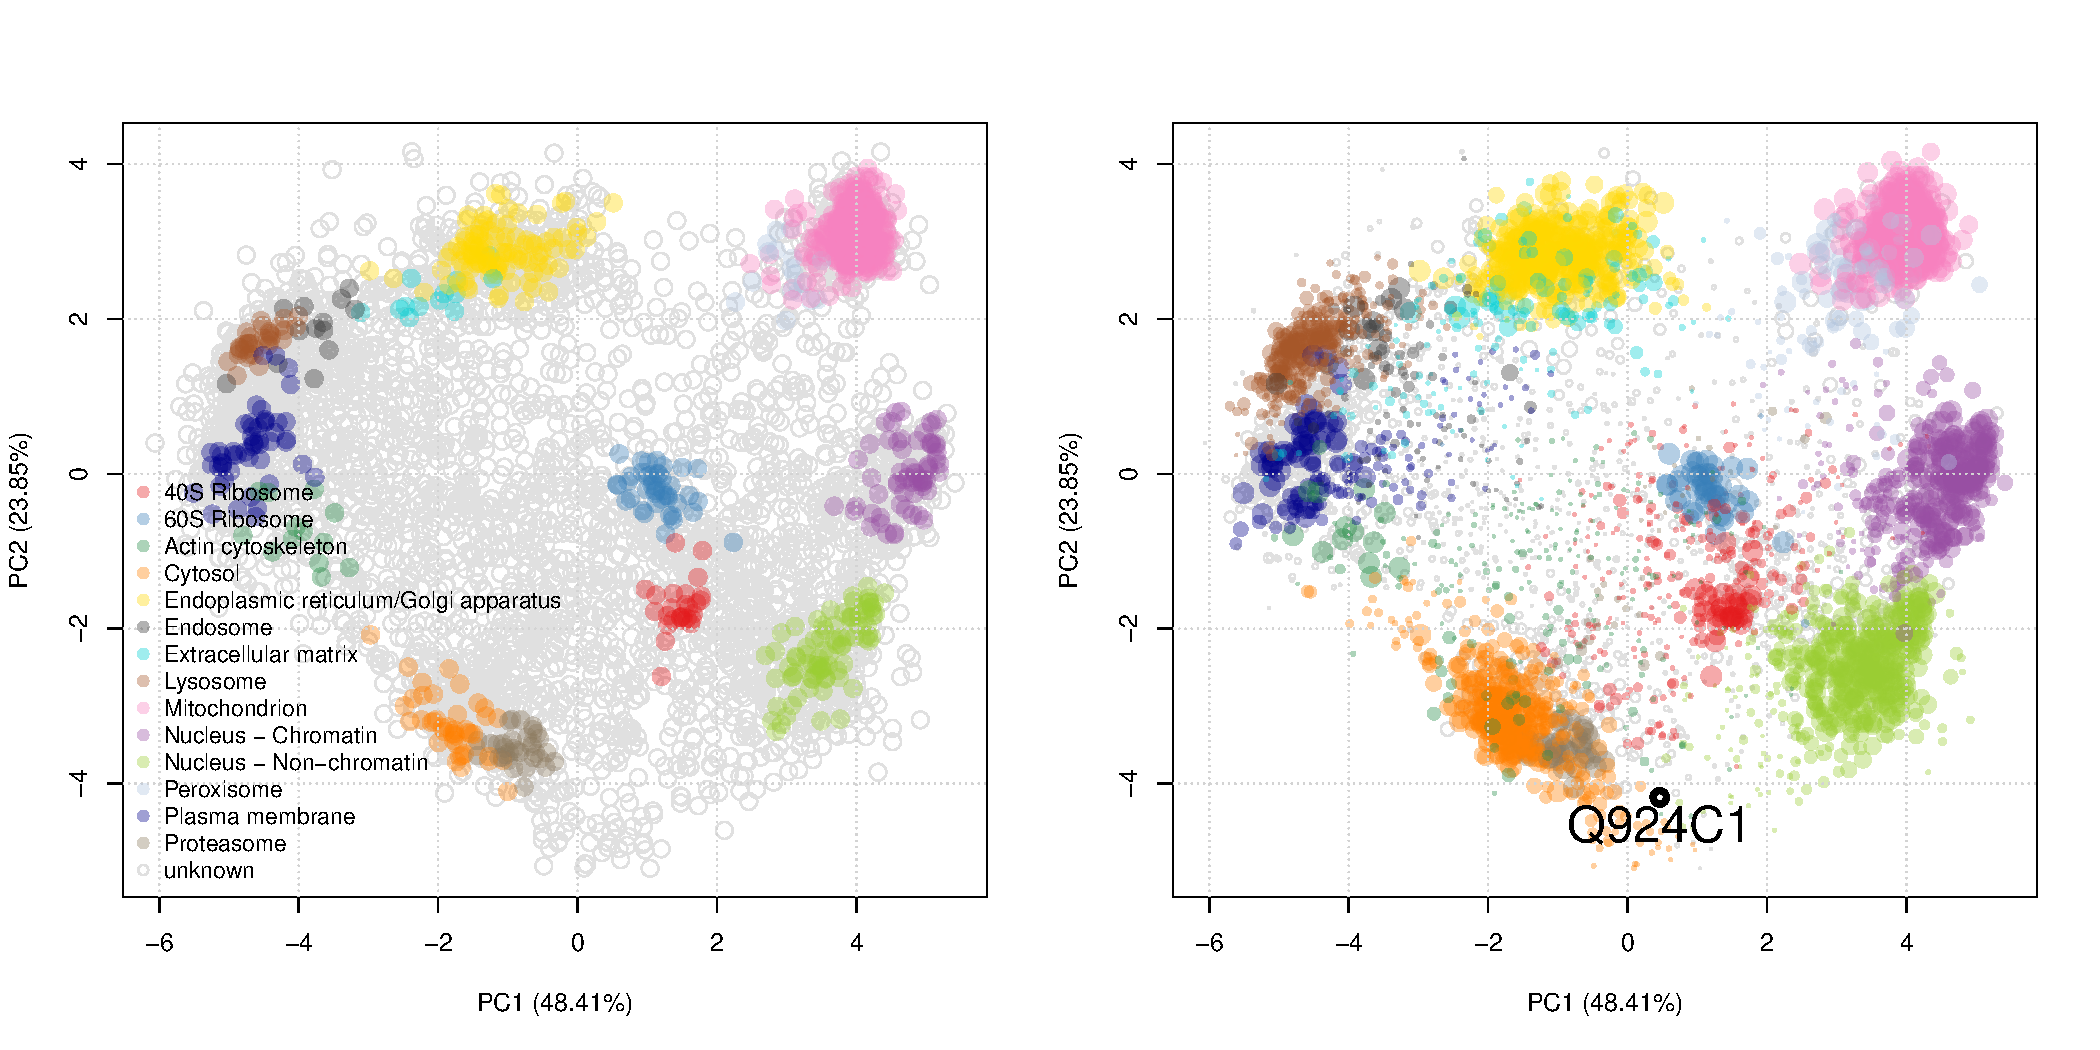
\includegraphics[width=1\linewidth]{./figs/tagm_pca_res.pdf}
        \caption{Assignment of proteins of
          \textit{unknown} location to one of the annotated
          classes. The dots are scaled according to the protein
          assignment probabilities.}
      \end{figure}
\end{frame}

\begin{frame}{}
  \begin{figure}
    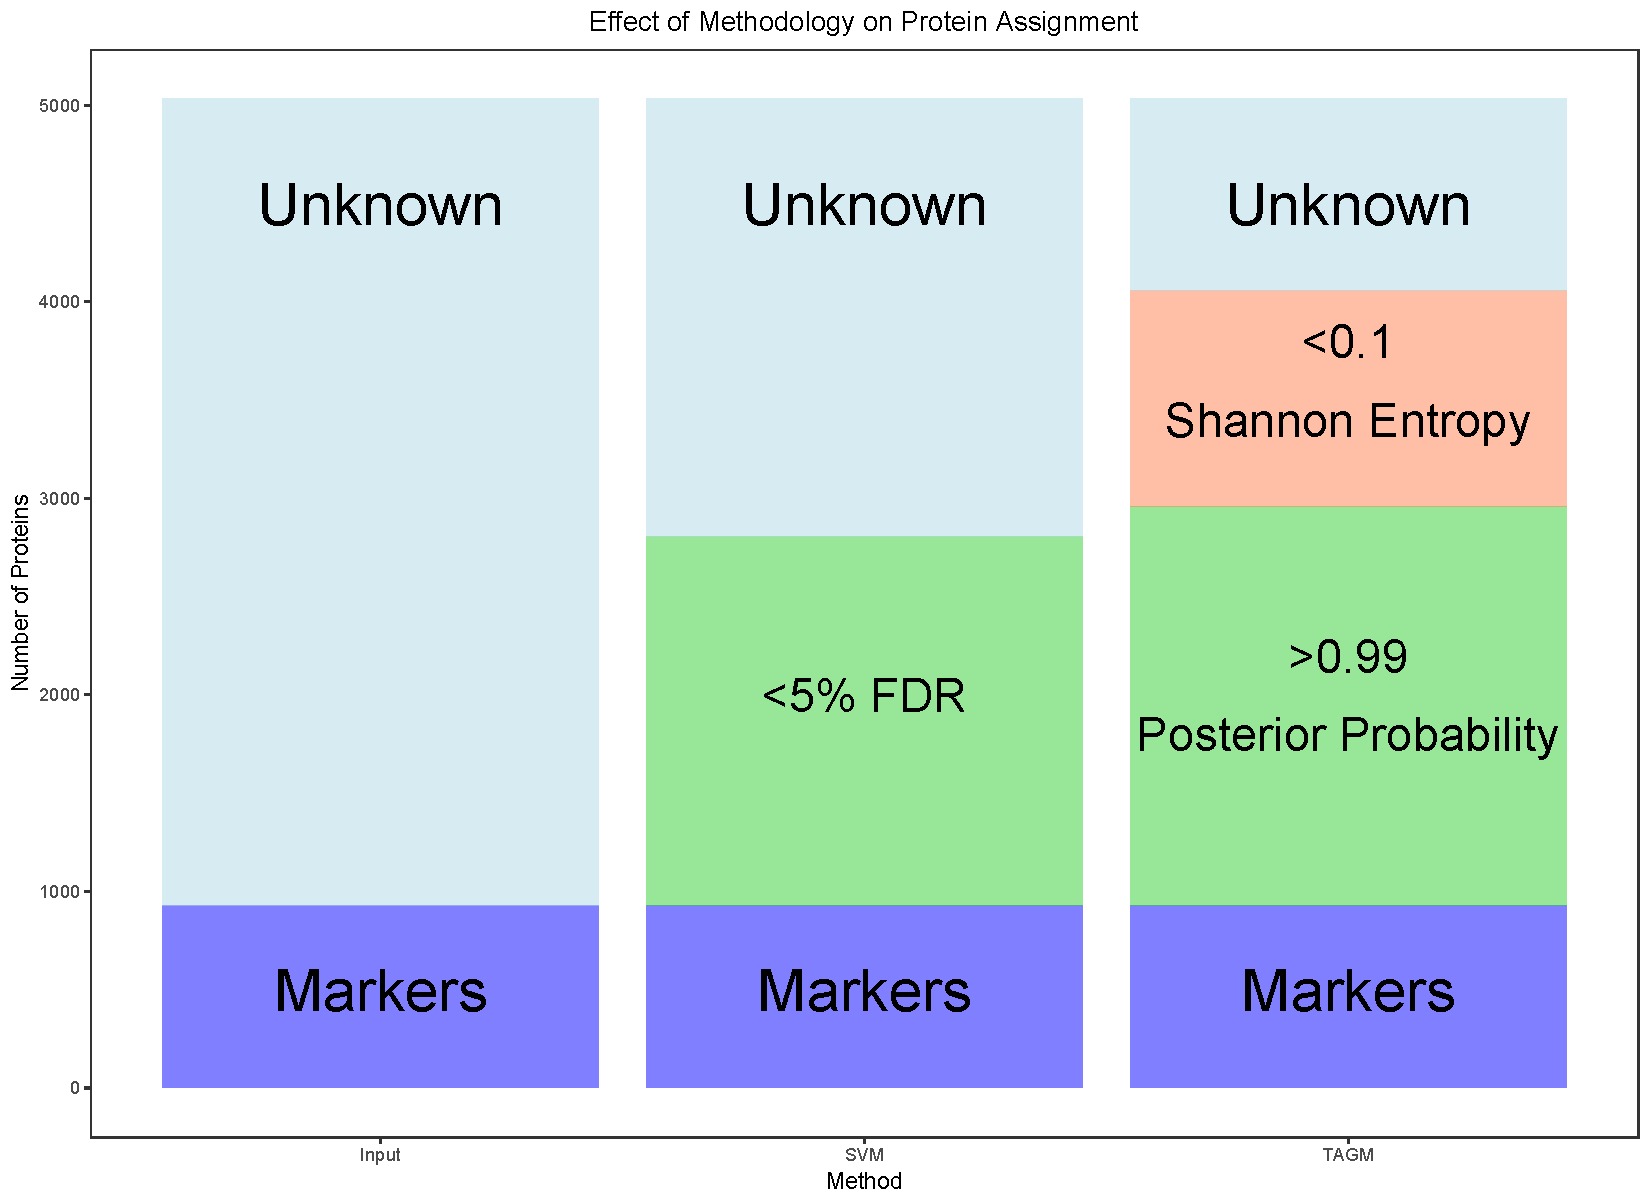
\includegraphics[width=.8\linewidth]{./figs/ConcludePlot.pdf}
  \end{figure}
\end{frame}

\begin{frame}
  \begin{figure}
    \centering
    \sidebysidecaption{0.55\linewidth}{0.42\linewidth}{
      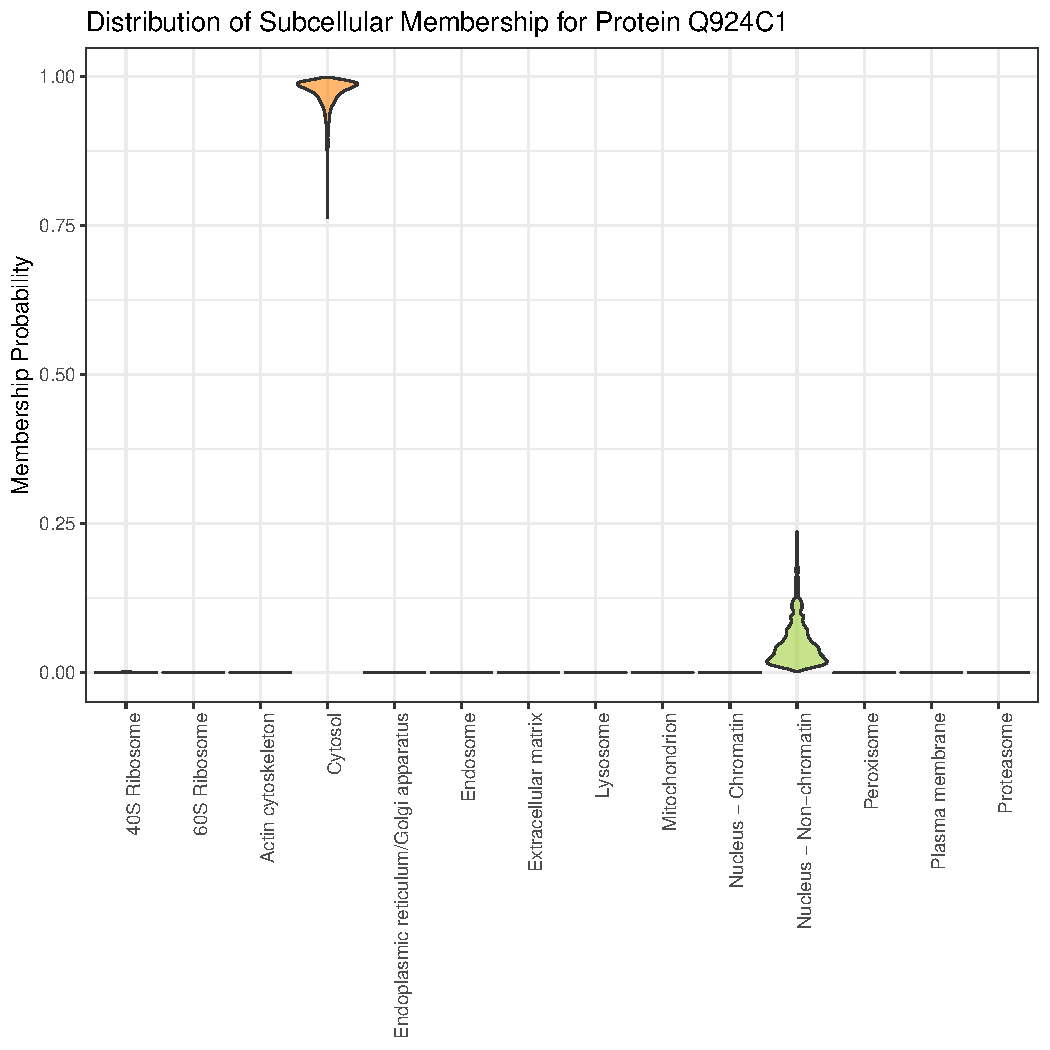
\includegraphics[width=1\linewidth]{./figs/Q924C1-prob-1.pdf}
    }{
    \caption{\scriptsize \justifying Exportin 5 (Q924C1) forms part of
      the micro-RNA export machinery, transporting miRNA from the
      nucleus to the cytoplasm for further processing.  It then
      translocates back through the nuclear pore complex to return to
      the nucleus to mediate further transport between nucleus and
      cytoplasm. The model correctly infers that it most likely
      localises to the cytosol but there is some uncertainty with this
      assignment. This uncertainty is reflected in possible assignment
      of Exportin 5 to the nucleus non-chromatin and reflects the
      multi-location of the protein.}  }
    %% NOTE SVM failed to classify exportin 5 to any of the two
    %% biologically plausible locations, arguably due to the similarity
    %% of the cytosol and peroxysome, to which it got assigned.

  \end{figure}
\end{frame}


\begin{frame}{Whole sub-cellular proteome uncertainty}
  \begin{figure}
    \centering
    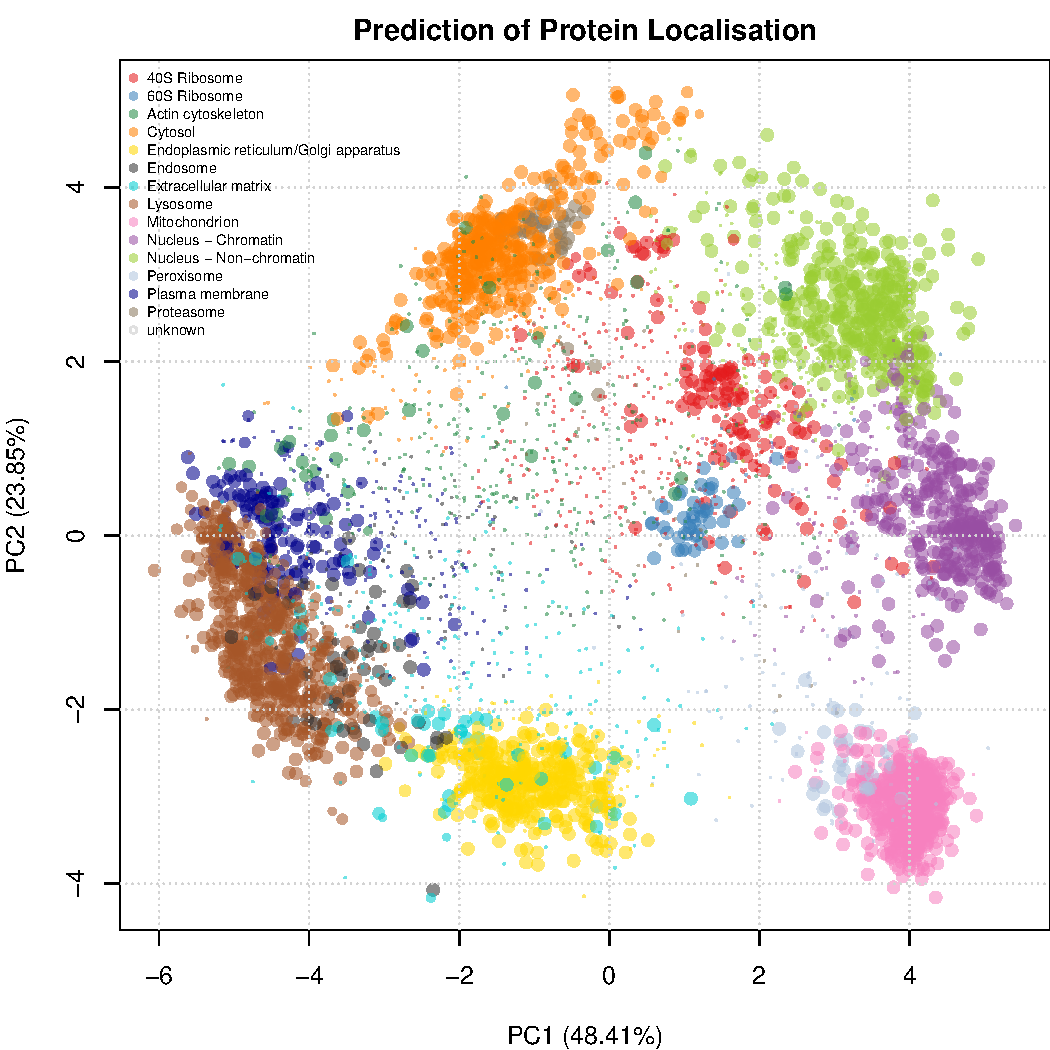
\includegraphics[width=.32\linewidth]{./figs/pca-tagm-mcmc-1.pdf}
    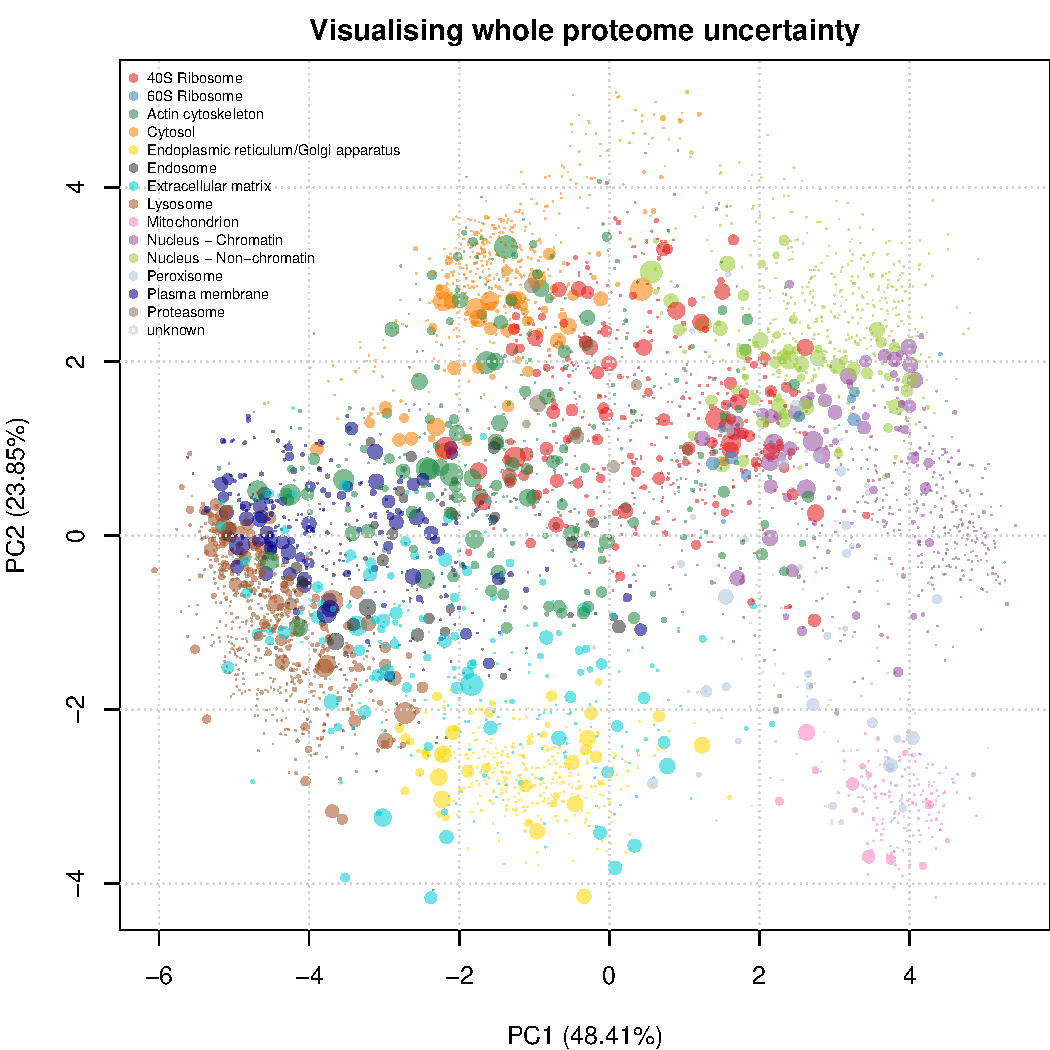
\includegraphics[width=.32\linewidth]{./figs/pca-tagm-map-1.pdf}
    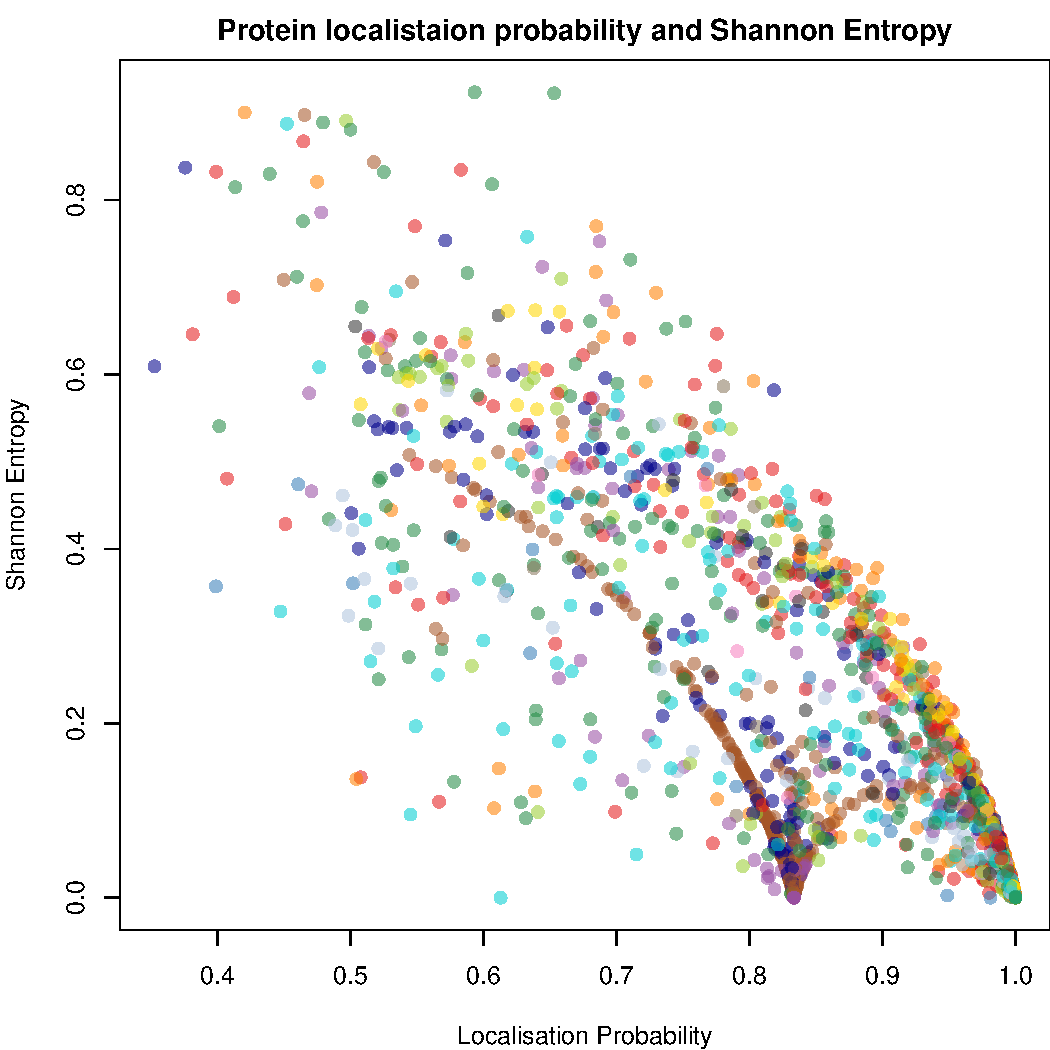
\includegraphics[width=.32\linewidth]{./figs/prob-vs-shannon-1.pdf}
  \end{figure}
\end{frame}


%-----------------------------------------------
% New section
%-----------------------------------------------

\subsection{Spatial dynamics}


\begin{frame}{Spatial dynamics}
  \begin{figure}[h]
    \centering
    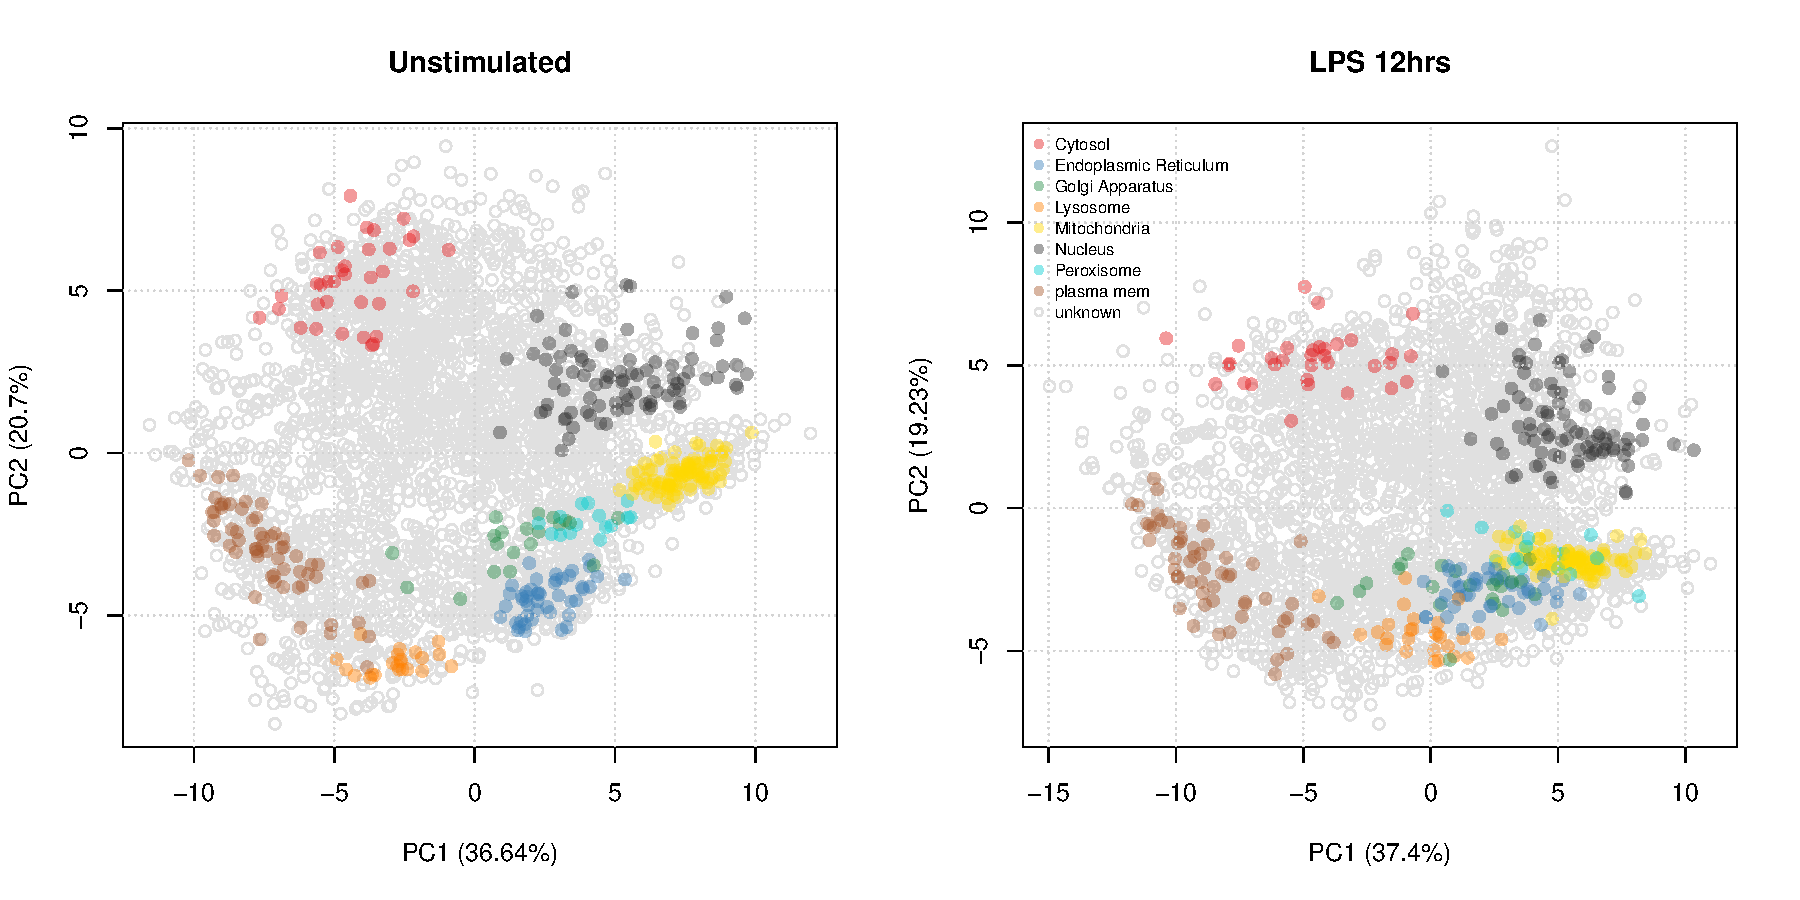
\includegraphics[width=\linewidth]{./figs/lps.pdf}
    \caption{Spatial maps of unstimulated (\textbf{control}) and
      LPS-treated (\textbf{experimental condition}) cells (combined
      triplicates).}
  \end{figure}
\end{frame}


\begin{frame}
  A probabilistic definition of differential localisation:

  \begin{align}
    {x}_i = p ( z_{i, 1} \neq z_{i, 2} )
  \end{align}

  with

  \begin{itemize}
  \item organelle-specific profiles modelled with mixtures of
    non-paramateric distributions \citep{Crook:2019b};
  \item explicit modelling of replicates and their variability;
  \item no assumption with regard to similarity of gradients between
    conditions;
  \item rigorous interpretation of the results with uncertainty
    quantification of differential localisation.
  \end{itemize}

\end{frame}


\begin{frame}
  \begin{figure}[h]
    \centering
    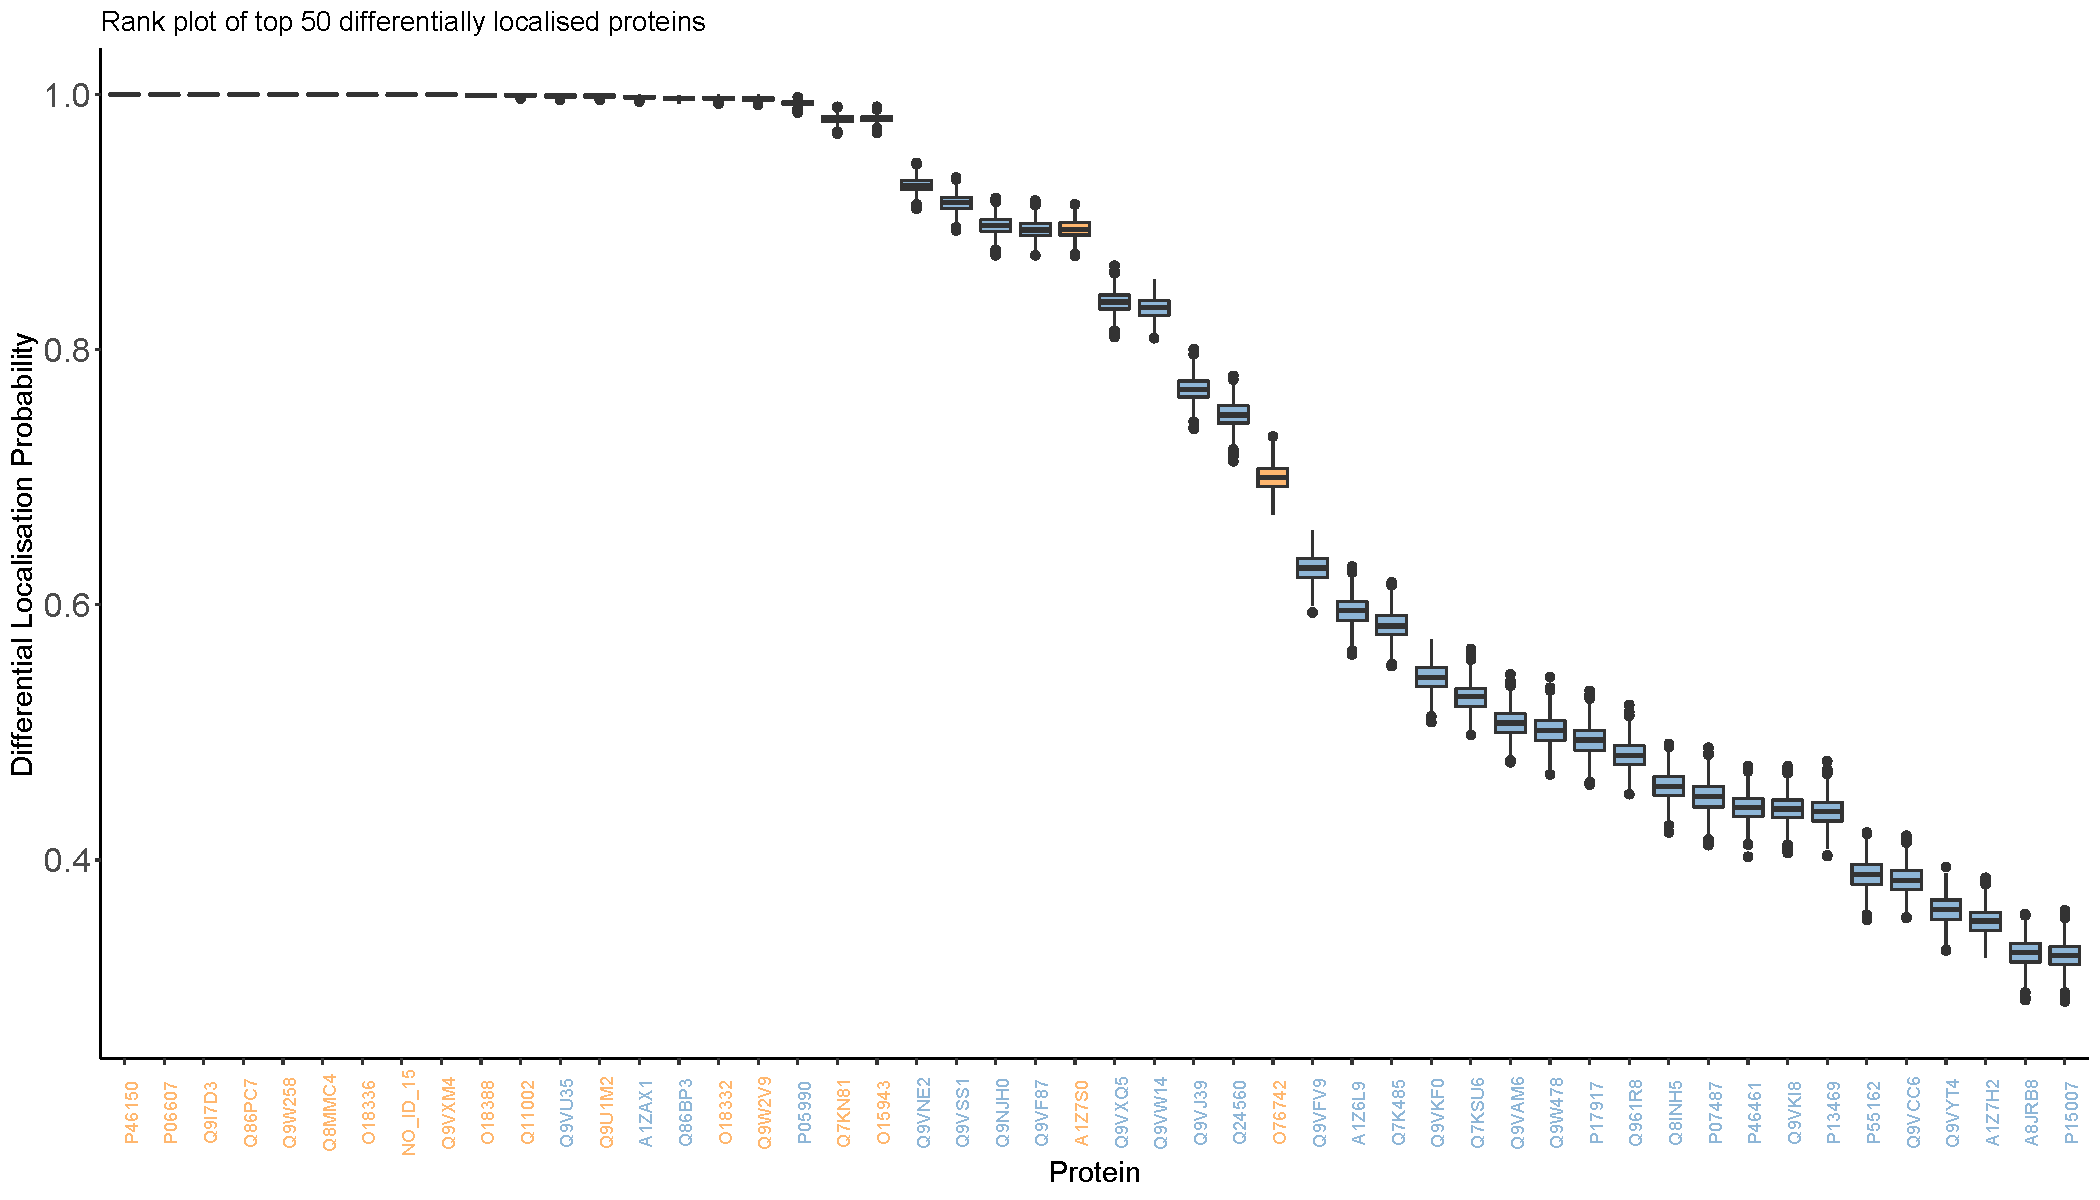
\includegraphics[width=\linewidth]{./figs/rankboxplot.pdf}
    \caption{Proteins ranked based on their probability of being
      differentially localised, i.e. having been assigned different
      niches in the control and experimental condition. Orange: TP,
      blue: FP.}
  \end{figure}
\end{frame}


\begin{frame}
  \begin{figure}[h]
    \centering
    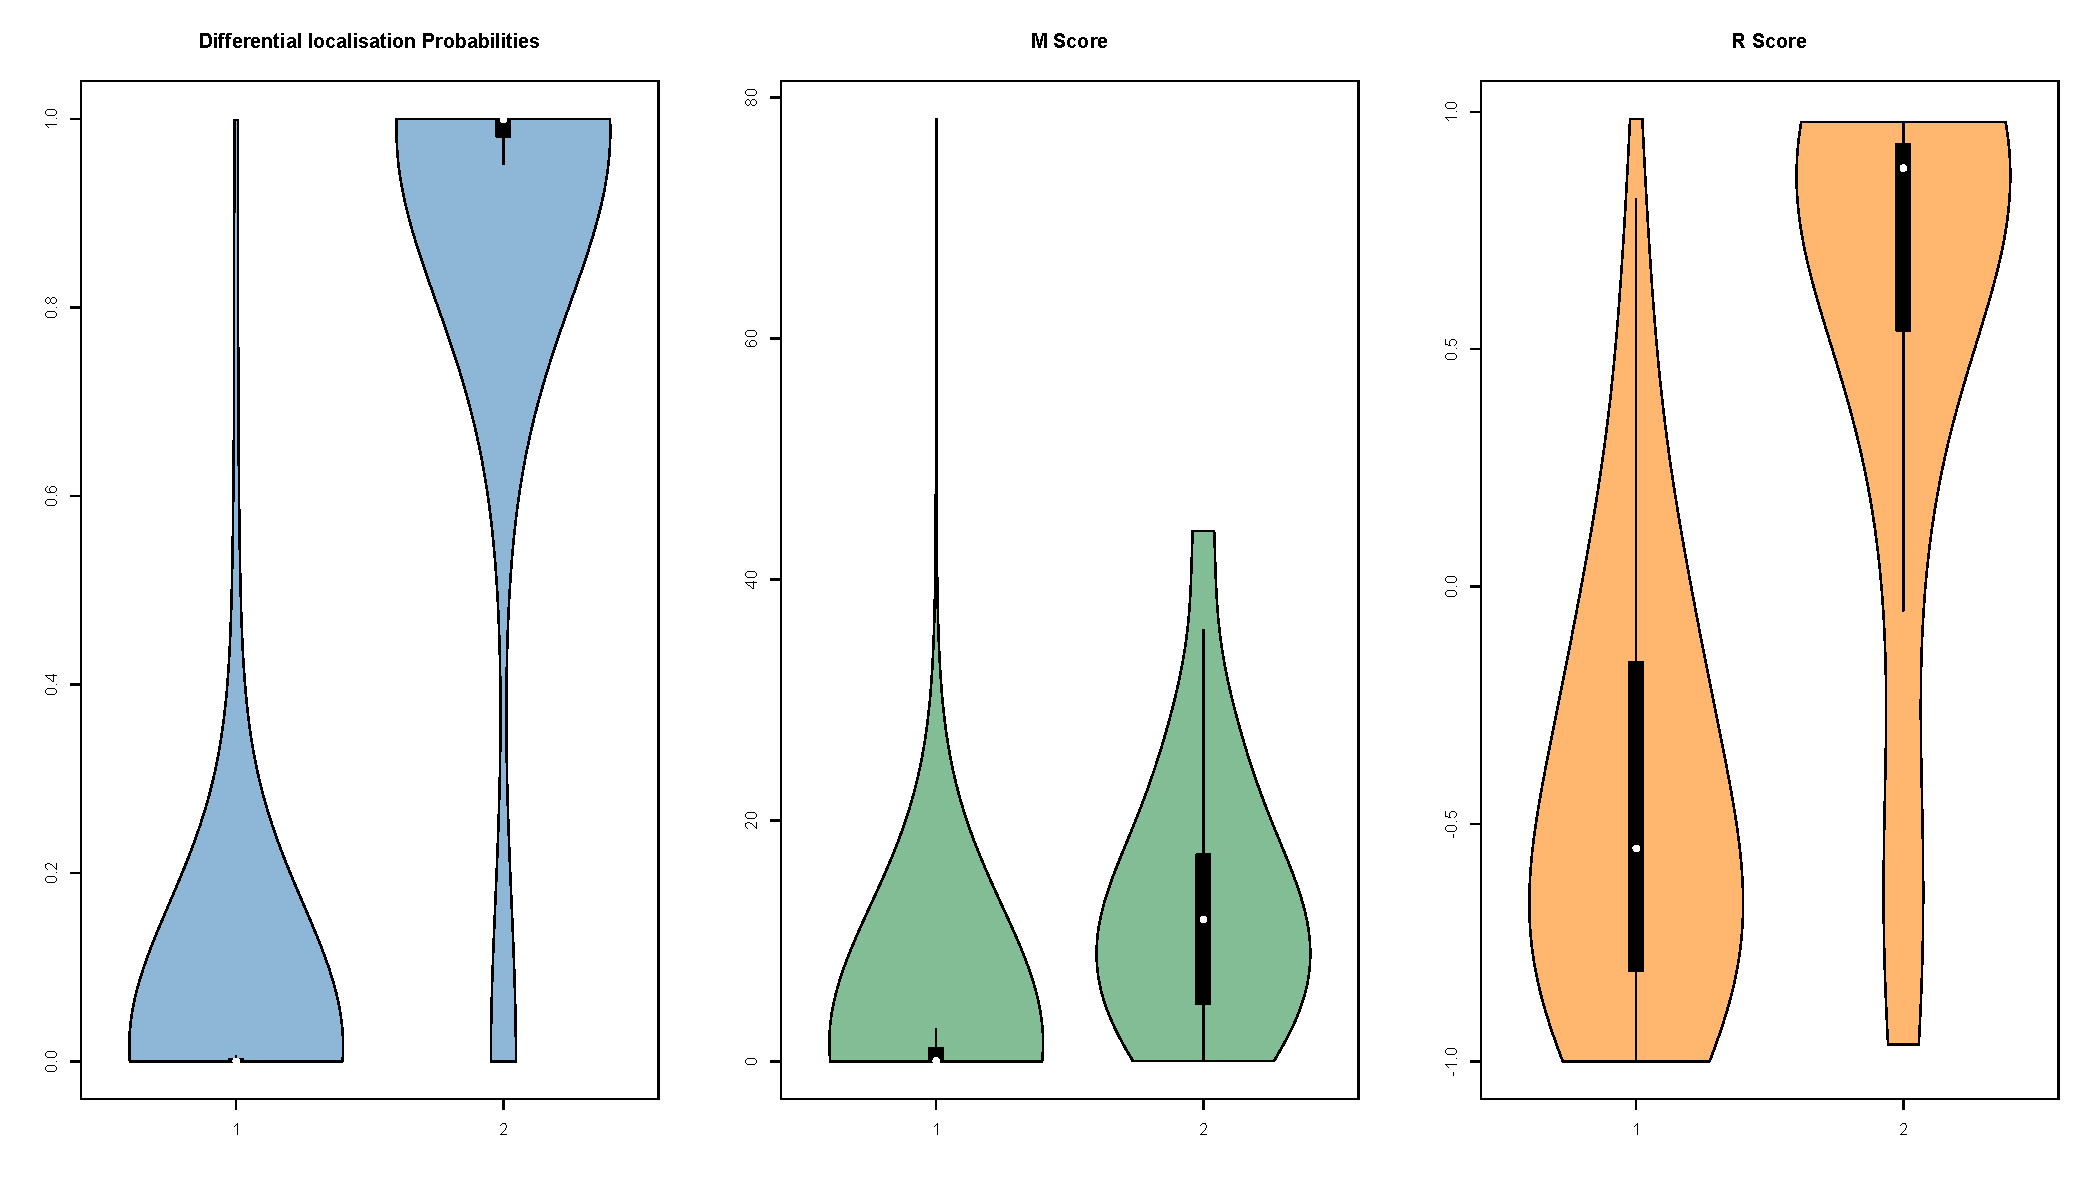
\includegraphics[width=\linewidth]{./figs/vioplotInformative.pdf}
    \caption{\textbf{\textcolor{Blue}{Differential localisation
          probabilites}} (\textbf{left}) provide excellent
      discrimination betwee static (1) and differentially localised
      proteins (2).}
  \end{figure}
\end{frame}


%-----------------------------------------------
% New section
%-----------------------------------------------

\section{Behind the scences}


\begin{frame}{}
  \begin{center}
    \Large{\textbf{Behind the scenes}:
      \textcolor{Blue}{\textbf{Applied} Bioinformatics} Life Sciences -
      software/data structures and open research practice.}
  \end{center}
\end{frame}


\begin{frame}{}

  Beyond the figures\footnote{... which are all reproducible, by the way.}

  \begin{itemize}
  \item Software: \textbf{infrastructure}
    (\href{http://bioconductor.org/packages/MSnbase}{\texttt{MSnbase}},
    \cite{Gatto:2012}), \textbf{dedicated machine learning}
    (\href{http://bioconductor.org/packages/pRoloc}{\texttt{pRoloc}},
    \cite{Gatto:2014a}), \textbf{interactive
      visualisation}\footnote{\url{https://lgatto.shinyapps.io/christoforou2015/}}
    (\href{http://bioconductor.org/packages/pRolocGUI}{\texttt{pRolocGUI}},
    \cite{pRolocGUI}) and \textbf{data}
    (\href{http://bioconductor.org/packages/pRolocdata}{\texttt{pRolocdata}},
    \cite{Gatto:2014a}) for spatial proteomics.
  \item The \href{http://bioconductor.org/}{\textbf{Bioconductor}}
    \citep{Huber:2015} ecosystem for high throughput biology data
    analysis and comprehension: \textbf{open source}, and
    \textbf{coordinated and collaborative\footnote{between and within
        domains/software} open development}, enabling
    \textbf{reproducible research}, enables understanding of the data
    (not a black box) and \textbf{drive scientific innovation}.
  \end{itemize}
\end{frame}


%-----------------------------------------------
% New section
%-----------------------------------------------

\section{Conclusions}


\begin{frame}[fragile]{Conclusions}
  \begin{itemize}
  \item \textcolor{Blue}{Applied Bioinformatics}: Reliance on
    computational biology, statistics and dedicated software
    (\texttt{pRoloc} \textit{et al.}) to interpret data and acquire
    biological knowledge.
  \item \textcolor{Blue}{Life Sciences}: Protein sub-cellular
    localisation, technologies (hyperLOPIT) and opportunities.
  \item Rigorous computational infrastructure and sound data analysis
    and interpretation is a \textcolor{Blue}{\textbf{long term
        investment}}.

  \end{itemize}

\end{frame}



%-----------------------------------------------
% References
%-----------------------------------------------


\begin{frame}[allowframebreaks]{References}
  \scriptsize
  \bibliographystyle{plainnat}
  \bibliography{refs}
\end{frame}


%-----------------------------------------------
% Final slide
%-----------------------------------------------

\begin{frame}%[noframenumbering]
%\thispagestyle{empty}

% Logo UCL a gauche
\begin{tikzpicture}
  \useasboundingbox (0,0) rectangle(\the\paperwidth,1);
  \node[inner sep=0pt] at (1.7,2) {
\includegraphics[width=.33\textwidth]{UCL_2018}};
 \end{tikzpicture}
\vspace{.1cm}



\begin{center}
  \textbf{Thank you for your attention}
\end{center}


\bigskip

\begin{center}
  \textbf{laurent.gatto@uclouvain.be} – de Duve Institute \\
  \url{lgatto.github.io/about} \\
  Slides available at \textbf{\url{http://bit.ly/ABLS2020}}.
\end{center}

\end{frame}


\end{document}
